\subsection{CONCERT} \label{concert}




CONCERT on virtualisointiin keskittyvä mobiiliverkon ja reunalaskennan arkkitehtuuri \cite{liu2014concert}.
Nykyinen LTE-verkko kostuu joukosta erilaisia laitteita, joilla jokaisella on jokin spesifi tehtävä.
CONCERT pyrkii virtualisoinnilla vähentämään tällaisten laitteiden määrää.
Kyseessä on siis NFV:tä hyödyntävä ratkaisu.
Ehdotuksen tavoitteena on että virtualisoinnille yleiset hyödyt pätisivät myös tässä.
Tavoitteena on että toimintojen käyttöönotto olisi vähemmän riippuvainen fyysisiten laitteiden asentamisesta, toimintojen tuottamiseen käytettävät resurssit skaalautuisivat paremmin ja että resurssien käyttöaste olisi parempi.
Näiden tavoitteiden ehtona on käytännössä kaikkien mobiiliverkon toimintojen muuntaminen ohjelmalliseen muotoon ja virtualisoida ne.
Tämä pätee kaikkiin laitteisiin alkaen tukiasemista ja edeten aina EPC:n komponentteihin asti.
Koska muutos on suuri, CONCERT:n tavoitteena on seuraavan sukupolven mobiiliverkko, eikä integraatio nykyisiin mobiiliverkkoihin.
CONCERT:n idea on pääpiirteittäin yhdenmukainen ETSI:n NFV näkemyksen \cite{etsinfv5g} kanssa, NFV:n hyödyntämisestä viidennen generaation mobiiliverkkojen yhteydessä.

\begin{figure}[tb]
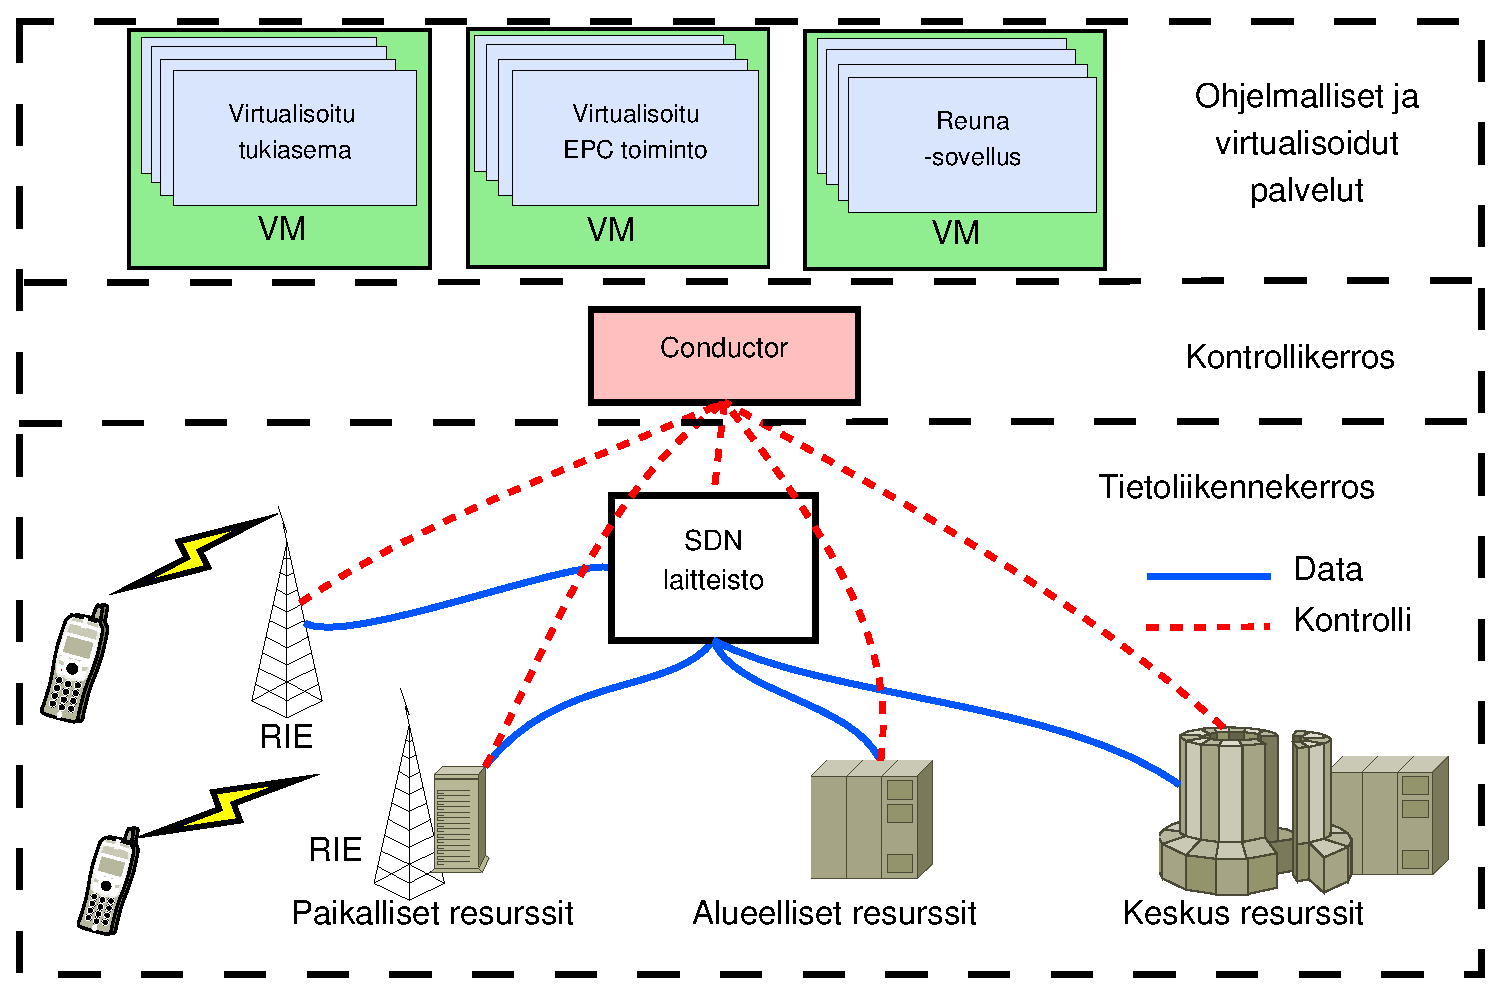
\includegraphics[width = \textwidth]{CONCERT.eps}
\caption{CONCERT arkkitehtuuri. Mukaelma julkaisussa \cite{liu2014concert} esitetystä kuvasta} \label{fig:concert}
\end{figure}

Yleisen palvelinlaitteiston hyödyntäminen palveluiden tuottamiseen mahdollistaa useiden eri toimintojen sijoittamisen virtualisoituina samaaan fyysiseen laitteistoon.
CONCERT ehdotuksen on tuottaa sekä mobiiliverkon toiminnallisuudet, että reunapalvelut samalla laitteistolla. 
Mobiiliverkon toimintojen virtualisointia on ehdotettu ennenkin. Esimerkiksi kappaleessa \ref{nfv} käsiteltiin C-RAN tyyppistä ehdotusta. C-RAN tavoitteena on virtualisoida tukiaseman toiminnalliset osat, siten että ne voitaisiin keskittää virtualisoituina palvelinsaleihin. 
CONCERT:n mukaan tämänkaltainen ratkaisu johtaisi liiallisesti keskitettyyn ja fyysisesti kaukana sijaitsevaan toteutukseen, jossa reunalaskennan tai muiden lyhyistä viiveistä riippuvaisten palveluiden toteuttaminen ei onnistuisi \cite{liu2014concert}. Lisäksi CONCERT haluaisi tukiasemien toimintojen lisäksi virtualisoi nykyisen EPC:n alaiset toiminnot.
CONCERT ehdottaa liiallisen keskittämisen välttämisesksi resurssien sijoittelua hierarkiseen malliin.
Kolmetasoisen hierarkian resurssit on jaettu kolmeen tasoon: paikalliseen, alueelliseen ja keskus. 
Paikallisen tason resurssit olisivat kaikkein vähäisimmät ja ne sijatsisivat tukiasemien välittömässä yhteydessä.
Aluellisen tason resurssit olisivat suuremmat kuin paikallisen ja sijaitsisivat kauempana.
Keskus tason resurssit olisivat kaikkein suurimmat, mutta sijaitsisivat kaikkein kauimpana. 
Hierarkisen rakenteen ansiosta kaikkein tiukimman aikavaatimuksen sisältävä reunalaskenta voidaan suorittaa lähimmillä resursseilla ja muu laskenta välittää kauempana sijaitseville resursseille.

CONCERT jakaa järjestelmän kontrolli- ja tietoliikennekerrokseen (control/data plane). 
Tietoliikennekerros koostuu mobiiliverkon ja reunalaskennan mahdollistavasta laitteistosta, joka sisältää palvelinresurssit, radioliikenteestä vastaavan laitteiston (Radio Interfacing Equipment, RIE) sekä SDN kytkimistä. Huomautettakoon että RIE vastaavanlainen toimija kuin C-RAN ehdotuksen RRH.
Tietoliikennekerroksella on edellä kuvattu hierarkinen rakenne, jonka sisäisestä tietoliikenteen välittämisestä vastaa SDN.
Kontrollikerroksen ainoana toimijana on conductor, joka vastaa CONCERTin hallinnollisista toimista.
Reunalaskennan kannalta merkityksellisenä toimintona conductorissa on LCM (Locatio-Aware Computing Management).
LCM vastaa reunalaskentaan liittyvien resurssien hallinnasta. Tämä sisältää esimerkiksi käytettävien reunaresurssien osoittamisen reunalaskennan aikavaatimuksien ja mahdollisten resurssi vaatiumuksien mukaan.
Lisäksi kontrollikerroksen tehtävänä on lisäksi konfiguroida SDN reititykset siten että reunapalvelut ovat saavutettavissa.

CONCERTin arkkitehtuurikuvaus sisältää maininnan virtualisoitujen palveluiden dynaamisesta migratoinninsta, mutta ei määrittele sen tarkempaa kuvausta sen toiminnasta. Voidaan kuitenkin olettaa että se kattaa reunalaskennan siirtämistä esimerkiksi tilanteissa joissa käytössä olevan reunasolmun resurssit eivät riitä tai aikavaatimuksiin voitasiin vastata paremmin jollain toisella sijainnilla.

Virtualisoinnin voidaan sanoa olevan CONCERT:n ydin. CONCERT hyödyntää virtualisointia mobiiliverkon toimintojen tuottamiseen ja reunalaskennan tarjoamiseen. Tämän mahdollistaa yhtenäiset resurssit molemmille, sekä vähentää tarvetta erillisille laitteitoille.
Hierarkkisen rakenteen avulla CONCERT tavoittelee parempaa resurssien käyttöastetta sekä  reunapalveluiden vaatimien aikavaatimuksien täyttämistä.
NFV, SDN ja mobiiliverkon toimintojen toteuttaminen ohjelmallisina ovat kaikki edellytyksiä CONCERT:n toteutumiseksi. Toistaiseksi kaikki näistä ovat vasta kehityksessä.
Kyseessä on kokonaisuudessaan hyvin suuri muutos mobiiliverkon toimintaan, eikä ainoastaan vanhojen toiminnallisuuksien uudellentoteutus virtuaalisina.
